
Up until now only standard measures like the Area Under Curve (AUC) have been used in order to quantify and balance the particular cases of misclassification. However, in a business setting such as this differen faulty categorizations are typically associated with different types of costs. So naturally, it is desirable to operate on these directly in order to minimize them. Unfortunately, this problem is in its essence non-continuous and as such it is not possible to compute the gradients directly. This necessitates the use of non-standard optimization techniques \cite{GAml}.

One such technique is to use the predictive framework of the Logistic Regression in conjunction with a Genetic Algorithm. The Genetic Algorithm tries to emulate an evolutionary process, where in the first step candidate coefficient vectors $\beta \in \mathbb{R}^d, d \in \mathbb{N}$ are randomly sampled and ranked with respect to the cost which results from their predicted probabilities $p(y=1|\beta)$ and a threshold $c$ that serves as a decision criterion, where

\begin{align*}
\hat{y} = \begin{cases}
  1 \quad if\ p(y|\beta) > c\\
  0 \quad else
\end{cases}.
\end{align*}

The most successfull candidates are then allowed to propagate and be combined to form the new set of candidate values for $\beta$ in the next iteration \cite{GAorigin}. An outline is given in pseudocode in algorithm \ref{GA}. One problem with this approach lies in its tendency to overfit. In order to mitigate this, two minor modifications where added. First, a random sampling technique was used, where the fitness of each candidate in the population was computed only by a small {\parfillskip0pt\par}

\begin{algorithm}
\tiny
\caption{Genetic Algorithm}
\label{GA}
\begin{algorithmic}
\State \texttt{history} $\gets$ []
\For{i in 1, ..., maxiter}
    \State \# Initialize/Reset lists
    \State \texttt{fitness} $\gets$ \texttt{repeat(}$-\infty$ \texttt{, population\_size)}
    \State \texttt{cutoffs} $\gets$ \texttt{repeat(} $-\infty$\texttt{, population\_size)}
    \If{\texttt{random()} $<$ \texttt{reset\_probability}}
        \State \texttt{X\_train}, \texttt{y\_train}, \texttt{price\_train} $\gets$ \texttt{resample()}
    \EndIf   
    \For{j, $\beta$ in \texttt{enumerate(population)}}
        \State \texttt{y\_pred} $\gets$ \texttt{predict\_proba(X\_train,}$\beta$\texttt{)}
        \State \texttt{fit, cut} $\gets$ \texttt{get\_fitness\_and\_c(y\_pred, y\_train, price\_train)}
        \State \texttt{fitness[j]} $\gets$ \texttt{fit}
        \State \texttt{cutoffs[j]} $\gets$ \texttt{cut}
    \EndFor
    \State \# Select the most fit individuals
    \State \texttt{fit\_idx} $\gets$ \texttt{argsort(-fitness)}
    \State \texttt{parents} $\gets$ \texttt{fit\_idx[0:num\_parents]}
    \State \# Overwrite population
    \State \texttt{population} $\gets$ \texttt{population[parents]}
    \State \# Crossover
    \While{\texttt{length(population) < num\_parents}}
        \State \texttt{parent\_a, parent\_b} $\gets$ \texttt{sample(population, 2)}
        \State \texttt{candidate} $\gets$ \texttt{crossover(parent\_a, parent\_b)}
        \If{\texttt{random() < mutation\_probability}}
            \State \texttt{candidate} $\gets$ \texttt{mutate(candidate)}
        \EndIf
    \EndWhile
    \State \# Store results
    \State \texttt{best} $\gets$ \texttt{argmax(fitness)}
    \State \texttt{history[i]} $\gets$ \texttt{population[best]}
\EndFor
\State \Return \texttt{argmax(history)}
\end{algorithmic}
\end{algorithm}



\noindent fraction of the available training data. This sample will be randomly redrawn in each iteration, which means that only solutions that generalize beyond many training sets have a chance to be propagated in the long term. Additionally this speeds up the run time of the algorithm and, fortunately, leads also to a better generalization overall \cite{garst}. Secondly, for the final result of the routine, instead of using the candidate $\beta$ that had the best fitness on the training data, the candidate is used that proved to have the highest fitness, i.e. the lowest cost on its respective out-of-bag-samples.

These modifications mean that it was not possible to use an out-of-the-box implementation for the Genetic Algorithm and it was necessary to write a custom built variant. On the positive side this allows for a very tailored approach to the problem. For example, when determining the fitness of a parameter vector $\beta$ the Logit Model will only provide probability estimates and the parameter $c$ for determining the predicted label of a particular case still needs to be tuned. In the custom implementation the fitness is evaluated for a particular realisation of $\beta$ on a whole grid of values for $c$. Afterwards the threshold for this particular $\beta$ is chosen such that it maximizes the fitness - as opposed to fix a threshold beforehand as a sort of hyperparameter.

\begin{figure}
\centering
\caption{Results of the Genetic Algorithm}\label{gaplot}
\begin{subfigure}[b]{0.5\textwidth}            
            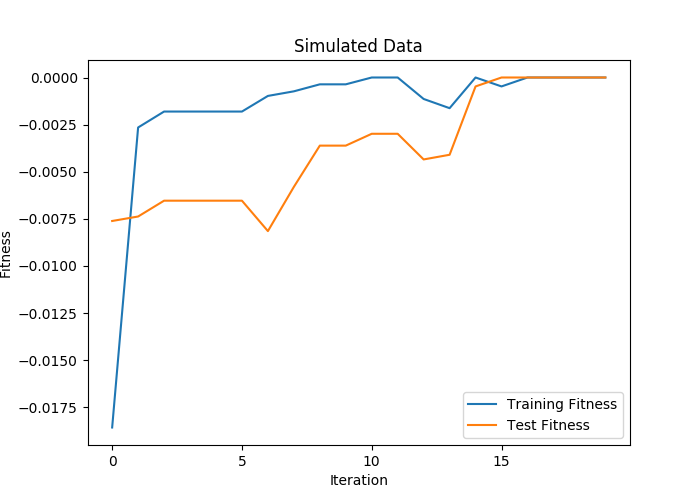
\includegraphics[width=\textwidth, height=110px]{%
            ../eda/genetic_test.png}
            \caption{Simulation}
    \end{subfigure}%
    \begin{subfigure}[b]{0.5\textwidth}
            \centering
            \includegraphics[width=\textwidth, height=110px]{%
            ../models/genetic_run_20190303_1029.png}
            \caption{Real but also fake}
    \end{subfigure}
\end{figure}


 In order to test the customized algorithm a simulation study was used. A data matrix $X$ was randomly initialized and a vector of known, 'true' coefficients $\beta_{true}$ was used to calculate deterministic true labels $y_{true}$ with the threshold $c_{true} = 0.7$ much in the same way as described above. The results of the simulation are described in the left part of figure \ref{gaplot}. The algorithm was able to find an approximate solution that was a scaled version of $\beta_{true}$ with a different threshold which provided a cost on the out-of-bag sample that was sufficiently close to zero. Having confirmed the reliabilty of the handcrafted routine in such a way it is possible to further assess the cost on the real data.

The Genetic Algorithm was executed multiple times with a different set of parameters for each run. Note however, that it was not possible to deploy a traditional grid search or a search by a tree of Parzen Estimators, with sufficient trials, due to the excruatiatinlgy long run times of the algorithm. Instead, four different configurations have been predetermined based on the insights provided by the simulation study and the experiment that provided the most promising results on their respective out-of-bag samples were used for the final predictions.

In particular, different methods for the crossover have been investigated, such as the \emph{arithmetic, point} and \emph{heuristic} crossover. 